\chapter{Technological Research}\label{cha:research}

\section{Overview}

This chapter presents the results of the initial technological research done to carry out the project. In here, the different technologies used in the project are explained in detail, as well as the benefits of using them and the reasons for doing so.

The list of tools and frameworks used on the project is the following:

\begin{itemize}
	\item RDF
	\item OWL
	\item SPARQL
	\item GeoSPARQL
	\item NodeJS
	\item AngularJS
	\item Leaflet
	\item Phonegap
	\item GPX
	\item GeoJSON
\end{itemize}

\section{RDF}

RDF stands for Resource Description Framework, and it is a framework for expressing information about resources. These resources can be anything, documents, people, physical objects, even abstract concepts.

RDF is intended for situation in which data is to be processed by machines and not simply displayed to humans, due to this, it is very useful for the goals of the Semantic Web. It can be used to publish and interlink data on the web. For example, retrieving a resource which represents a person, say Bob, could provide us with the fact that Bob knows another person, say, Alice, who is represented by her URI. Retrieving the resource representing Alice may then yield links to datasets about other persons and so on. A computer can automate this process and follow these links, aggregating data from different resources. This kind of uses are often known as Linked Data \cite{rdfprimer11}. 

There are many reasons to choose using RDF, the following are some of them:

\begin{itemize}
	\item Adding machine readable information to Webpages. This allows them to be displayed in enhanced format or to be processed by roaming agents.
	\item Enriching datasets by linking them to other sources of data.
	\item Interlinking APIs so that clients are able to discover new sources of information.
	\item Using the datasets currently published as Linked Data 
	\item Providing a standards compliant way of exchanging data between applications.
	\item Interlinking various datasets within an organization and allowing cross-dataset queries by using SPARQL.
\end{itemize}

\subsection*{RDF data model}

Data in RDF is formed by statements. This statements are called \textit{triples} and follow a subject-predicate-object structure. A statement on RDF represents a relationship between two resources, the \textbf{subject} and \textbf{object} represent the resources being related while the \textbf{predicate} represents the nature of the relationship. These relationships are phrased in a unidirectional way, from subject to object, and are called properties.

The same subject is often referenced in multiple triples and can of course be the object of other triples. These ability to have the same resource as subject and object in different triples makes it possible to find connections between RDF resources and is one of the most powerful features of the framework. A set of triples can be viewed as a connected \textbf{graph}, in figure \ref{fig:rdfgraph} we can se an example of a set of triples in pseudo-code and the graph representing them.

\begin{figure}[h]
  \centering
  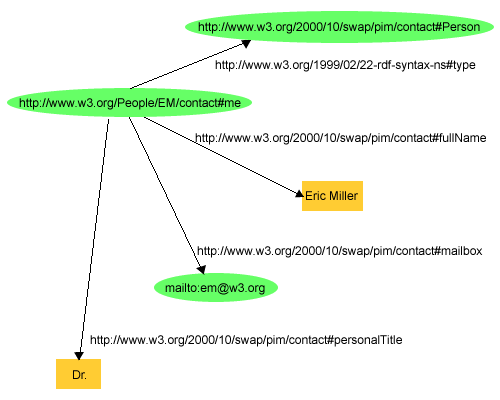
\includegraphics[width=.6\textwidth]{fig/rdfgraph}
  \caption{A set of triples and their corresponding graph}
  \captionsetup{font={footnotesize,bf,it}}
  \caption*{source: \url{http://www.w3.org/TR/rdf11-primer/}}
  \label{fig:rdfgraph}
\end{figure} 

There are three types of RDF data that can occur in triples: IRIs, Literals or Blank nodes \cite{rdfprimer11}.

\subsubsection*{IRIs}

IRI is an abbreviation for International Resource Identifier, which is used to identify a resource. On RDF, IRIs may appear in any component of triples, be it subject, object or predicate. The URLs (Uniform Resource Locators) which identify web pages are a form of IRI, however other forms of IRI can identify a resource without specifying its location. An IRI is a generalization of URIs allowing the use of non-ASCII characters unlike the latter. Thus, an IRI is defined as a set of characters unreserved characters which can include characters of the UCS \cite{rfc3986,rfc3987}(Universal Character Set, [ISO10646]).

An example of a IRI from dbpedia can be the following: \url{http://dbpedia.org/resource/Leonardo_da_Vinci}. Even if RDF does not explicitly specify what a certain IRI represents, they can take meanings from vocabularies or conventions.

In SPARQL (see \ref{sec:sparql}) and in some RDF serialization models prefixes can be defined. A dataset, for example http://example.org, could be given the name \textit{my}. By giving this name we can reference http://example.org/Bob, a resource on the dataset as my:Bob. This is useful for it helps to avoid clutter on the query and helps human understanding, thus, from now on, prefix notation will be used to express datasets and vocabularies on the document.

\subsubsection*{Literals}

Literals are the basic values that are not IRIs. Literals are associated with data types, for example, the \textit{Integer} and \textit{Float} data types are equivalent to the traditional types from the programming languages. The string typed literals may optionally have a language associated allowing internationalization. Most of the regularly used data types are defined by XML Schema\cite{xmlschema}.

One particularity of RDF data types is that they can be defined on ontologies. Due to this, it is possible to find custom types, such as a string representing the serialization in WKT\cite{wkt} format of a geometry. 

An example of different types of triples, including literals can be found in listing \ref{lst:triplesliterals}.

\begin{listing}\centering
  \begin{minipage}{.6\textwidth}
    \begin{minted}[linenos=true,mathescape,gobble=6]{xml}
      <my:Bob> <foaf:name> "Bob"
      <!--The object is a literal of type String -->
      <my:Bob> <rdf:type> <foaf:Person> 
      <my:Bob> <foaf:age> "19"^^xsd:Integer 
      <!-- The literal is of type Integer -->
    \end{minted}
  \end{minipage}
  \caption{Different types of triple statements.}\label{lst:triplesliterals}
\end{listing}

\subsubsection*{Blank nodes}

Blank nodes are used to refer to resources who don't have or need a global identifier (an IRI). For example, we may want to refer to the right arm of a person, however, we may think that it is too verbose or unnecessary to actually give a identifier to this arm, so we could use a blank node to represent it, as illustrated in listing \ref{lst:triplesblanknode}. In this example it makes sense to have a blank node, for the right arm is directly dependent on the person, an arm (usually) makes no sense detached from a person.

\begin{listing}\centering
  \begin{minipage}{.6\textwidth}
    \begin{minted}[linenos=true,mathescape,gobble=6]{xml}
      <my:Bob> <rdf:type> <foaf:Person> 
      <my:Bob> <my:hasRightArm> :_b1
      :_b1 <rdf:type> <my:Arm>
    \end{minted}
  \end{minipage}
  \caption{Triple statements with a blank node.}\label{lst:triplesblanknode}
\end{listing}

\subsection*{RDF vocabularies}\label{ssec:rdfvocabularies}

The data model of RDF does not make any assumptions about the meaning of the IRIs representing the resources. However, in the reality, RDF is usually used in conjunction with a series of vocabularies or other conventions that give semantic information about these resources.

To allow the definition of vocabularies, RDF-schema\cite{rdfschema} is provided. This language allows the definition of RDF semantics, for example, one could define that the resource my:knows is a property or that the subjects of the previous triple are of type foaf:Person. RDF schema uses the concept of class, analogous to that on object oriented programming, to categorize resources. The property \textit{rdf:type} is used when specifying a class. This way, hierarchies of classes and sub-classes, properties and sub-properties can be defined. Domains and ranges can be also specified for properties, which specify the type of the subject and the object on these properties respectively. An example of RDF-schema can be found in listing \ref{lst:rdfschema}. There are alternatives for data modeling and inference to RDFS, such as OWL, however in many cases RDFS is enough to represent the logic on the system.

\begin{listing}\centering
  \begin{minipage}{.6\textwidth}
    \begin{minted}[linenos=true,mathescape,gobble=6]{xml}
      <foaf:Person> <rdf:type> <rdfs:Class> 
      <my:knows> <rdf:type> <rdf:Property>
      <my:knows> <rdfs:domain> <foaf:Person>
      <my:knows> <rdfs:range> <foaf:Person>
      <my:friendOf> <rdfs:subPropertyOf> <my:knows>
      :_b1 <rdf:type> <my:Arm>
    \end{minted}
  \end{minipage}
  \caption{Triple statements with a blank node.}\label{lst:rdfschema}
\end{listing}

RDF schema is not the only generally accepted vocabulary, there are several others that are currently considered standard. Among them we can find the following:

\begin{description}
	\item{Friend of a Friend (FOAF):} One of the first vocabularies used worldwide, it is used to represent persons, the properties that identify them and the relations among them \cite{foafspec}.
	
	\item{Dublin Core:} A metadata element set for describing a wide range of resources. Contains properties such as the creation date of the resource \cite{dublincorespec}.
	
	\item{schema.org: } A vocabulary for marking up web pages so that search engines can more easily find them \cite{schemaspec}.
\end{description}

\subsection*{Why RDF?}

Using RDF can greatly benefit this project. It can give a representation of the relationships on the system which can be easily analyses by machines. This can help building important functions, such as the recommendation system.

However, the use of RDF on this project is almost mandatory, for one of the goals is achieving data interoperability and publishing the data as Linked Open Data on the web.

\section{OWL}\label{sec:owl}

The Web Ontology Language (OWL) is a semantic markup language for publishing and sharing ontologies in the World Wide Web\cite{bechhofer2009owl}. The language is designed for applications that need to process the content of the information instead of just presenting it to humans. OWL provides greater machine interpretability than RDF or RDF schema by providing additional vocabularies along formal semantics.

OWL is used to explicitly represent the meaning of terms in vocabularies and the relationships among these terms. These representations are called ontologies\cite{mcguinness2004owl}. The standard is part of the stack of W3C recommendations for the semantic web, together with XML, XML Schema, RDF and RDF Schema.

OWL provides three sub-languages with increasing expressive power. Each subset of OWL includes all the previous ones, in addition to RDFS and RDF, so that there is no loss on expressive power as illustrated in figure \ref{fig:owlstack}.

\begin{figure}[h]
  \centering
  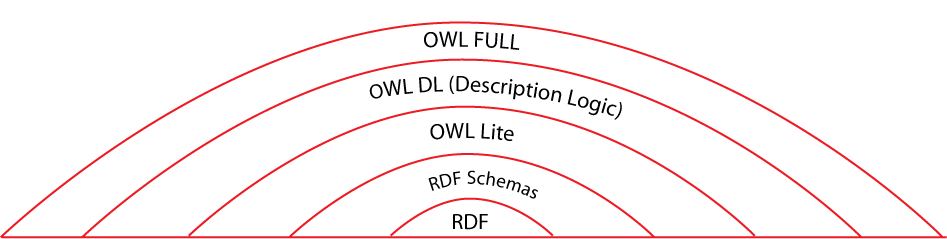
\includegraphics[width=.8\textwidth]{fig/owl-stack}
  \caption{The OWL levels of expressivity}
  \captionsetup{font={footnotesize,bf,it}}
  \caption*{source: \url{http://www.w3.org/}}
  \label{fig:owlstack}
\end{figure} 


\subsection*{OWL Lite}

OWL Lite is designed to support those users who need only a classification hierarchy and simple constraints. For example, while supporting cardinality constraints, it only allows cardinality 0 or 1, for the sake of simplicity. Due to this it should be simpler to provide tool support for OWL lite than to its other, more expressive, relatives. It also has a lower level of formal complexity than its more expressive siblings.

This sub-language contains all the features of RDF schema, such as category definitions through classes and hierarchical classification through subclasses, plus additional restrictions and expressions. OWL Lite provides tools for defining equality and inequality relations, property characteristics, property restrictions, restricted cardinalities and class intersections.

\subsubsection*{Equality and Inequality}

They are used to indicate equality and inequality relations among classes. One example

\begin{description}
\item[\texttt{equivalentClass}] Two classes may be stated as equivalents. This equality is used to create synonyms.

\item[\texttt{equivalentProperty}] It is used to define synonymous properties, the same way as with classes.

\item[\texttt{sameAs}] It states that two individuals are the same.

\item[\texttt{differentFrom}] The opposite to \texttt{sameAs}, used to indicate that two individuals are different. 

\item[\texttt{allDifferent}] It can ve used to state that a number of individuals are different from each other.
\end{description}

\subsubsection*{Property characteristics}

Property characteristics are special identifiers in OWL that provide information concerning the properties and their values. These characteristics are placed on properties, with relation to no class, as in listing \ref{lst:owl1}.


\begin{listing}\centering
  \begin{minipage}{.8\textwidth}
    \begin{minted}[linenos=true,mathescape,gobble=6]{xml}
      <owlx:ObjectProperty owlx:name="adjacentRegion" owlx:symmetric="true">
        <owlx:domain owlx:class="#Region" /> 
        <owlx:range owlx:class="#Region" />
      </owlx:ObjectProperty>
    \end{minted}
  \end{minipage}
  \caption{OWL property characteristic example.}\label{lst:owl1}
\end{listing}


\begin{description}
\item[\texttt{inverseOf}] Describes that a property is inverse to another. If A is related to B by the property P1 and P2 is the inverse of P1, then B will relate to A by property P2.

\item[\texttt{TransitiveProperty}] States that a property is transitive. For example, if A is related by transitive property P to B and B is related by P to C, then A will also be related by P to C.

\item[\texttt{SymmetrycProperty}] If a property is stated to be symmetric, then if A is related to B by the property, B will also by related to A by the same property.

\item{\texttt{FunctionalProperty}} If a property is functional, then it can have no more than one value for each individual. This mean that there will be no two triples of the same individual containing this property as a predicate.

\item[\texttt{InverseFunctionalProperty}] It states that the inverse of a property is a functional property.
\end{description}

\subsubsection*{Property restrictions}

OWL Lite allows to place restrictions regarding on how properties can be used inside of instances of classes. One example can be found in listing \ref{lst:owl2}

\begin{listing}\centering
  \begin{minipage}{.8\textwidth}
    \begin{minted}[linenos=true,mathescape,gobble=6]{xml}
      <owlx:Class owlx:name="Wine" owlx:complete="false">
        <owlx:Class owlx:name="&food;PotableLiquid" />  
        <owlx:ObjectRestriction owlx:property="#hasMaker"> 
          <owlx:allValuesFrom owlx:class="#Winery" />
        </owlx:ObjectRestriction> 
      </owlx:Class>
    \end{minted}
  \end{minipage}
  \caption{OWL property restriction example.}\label{lst:owl2}
\end{listing}


\begin{description}
\item[\texttt{allValuesFrom}] This restriction is placed on a property in relation to a class. It indicates that a property on a particular class has a local range restriction associated with it. For example, the class \textit{Person} may have a property \textit{hasDaugther}, restricted to have all values from class \textit{Woman}. This means that if an individual of type person is related by a relation \textit{hasDaugther} to other individual, we can infer that this individual will be a woman.

\item[\texttt{someValuesFrom}] This restriction is placed on a property in relation to a class. It indicates that at least one value from the property is of a certain type. For example, the class \textit{SemanticWebPaper} may have a property \textit{hasKeyword} restricted to have some values from \textit{SemanticWebTopic}. This would mean that a semantic web paper can have any number of keywords from any topic, as long as at least one of them belongs to a semantic web topic.
\end{description}

\subsubsection*{Restricted cardinalities}

OWL includes a limited form of cardinality restrictions. These are placed on properties with respect to classes, that is, the restrictions constrain the cardinality of the property in instances of a specific class.

\begin{description}
\item[\texttt{minCardinality}] If a minimum cardinality of 1 is stated on a property with respect to a particular class, then any instance of that class will be related to at least one individual by that property. For example, a person must have some sort of identifying card, thus, a minimum cardinality of 1 should be placed on the relation \textit{hasIDCard} with respect to \textit{Person}.

\item[\texttt{maxCardinality}] If a maximum cardinality of 1 is placed on a property with respect to a particular class, then any instance of that class will be related to at most one individual by that property. For example, a person should have at most one ID card, thus, the relation \textit{hasID} would have a maximum cardinality of 1.

\item[\texttt{cardinality}] It is used as a convenience to indicate that a property has both a maximum and a minimum cardinality with the same values. 
\end{description}

\subsubsection*{Intersection}

OWL Lite offers a very limited expressibility for intersections through the property \texttt{intersectionOf}. With this expression one could express that a \textit{EmployedPerson} is a intersection of a \textit{Employee} and a \textit{Person}. An example for this is shown in listing \ref{lst:owl3}

\begin{listing}\centering
  \begin{minipage}{.8\textwidth}
    \begin{minted}[linenos=true,mathescape,gobble=6]{xml}
      <owlx:Class owlx:name="WhiteWine" owlx:complete="true">
        <owlx:IntersectionOf>
          <owlx:Class owlx:name="#Wine" />
          <owlx:ObjectRestriction owlx:property="#hasColor">
            <owlx:hasValue owlx:name="#White" /> 
          </owlx:ObjectRestriction>
        </owlx:IntersectionOf>
      </owlx:Class>
    \end{minted}
  \end{minipage}
  \caption{OWL property restriction example.}\label{lst:owl3}
\end{listing}

\subsection*{OWL DL and OWL Full}

OWL DL is the second among the OWL sub-languages. It includes all the expressive power of OWL lite and adds on top of it. Similarly OWL Full adds on top of OWL DL. However, OWL Full is usually deemed as undecidable, in fact, there are no reasoners that can guarantee a solution in finite time. Due to this, many reasoners for OWL DL, such as Pellet try to find a way to convert OWL Full ontologies to a more a previous level of expressivity, since most ontologists use the highest expressive power when they only need OWL DL at most \cite{pellet}.

\subsection*{Why OWL?}

RDF schema provides a very limited way of expressing ontologies, it only allows to build classification hierarchies. Due to this, using OWL to describe the ontology would be the most recommendable thing. More specifically, the expression level of OWL DL, which allows to describe disjoint relations between classes (among other relation) plus all of the OWL Lite characteristics listed above, will allow to build a complete and correct ontology.
\section{SPARQL}\label{sec:sparql}

SPARQL is the recursive acronym for SPARQL Protocol and RDF Query Language. As its name indicates, it is a protocol and query language for RDF data. The idea behind this language is to allow the querying over RDF datasets in a similar language in which triples are expressed \cite{sparqlprotocol}.

SPARQL allows querying \cite{sparqlquery} and updating\cite{sparqlupdate} of RDF datasets. Similar to RDF, this language is composed of triples, however among the subjects predicates and objects, variables can be introduced. The logic behind SPARQL is stating a set of triples and introducing a variable somewhere among these triples. By doing so, the query engine will look and retrieve for all the cases which satisfy the set of triples in the query. Nothing impedes to query for a certain triple without specifying any variable, which can be useful when the goal is to know if the triple actually exists, but it is not the usual case.

In SPARQL prefixes can be used to indicate name spaces. By using the keyword prefix, it is possible to specify a URI which will be prepended to all triples using that resource. Variables are specified by using a interrogation mark (?) before an arbitrary name. Two examples can be found in listings \ref{lst:sparqlbasic} and \ref{lst:sparqlmedium}.

\begin{listing}\centering
  \begin{minipage}{.6\textwidth}
    \begin{minted}[linenos=true,mathescape,gobble=6]{sparql}
      SELECT ?s ?p ?o WHERE {
      	?s ?o ?o .
      }
    \end{minted}
  \end{minipage}
  \caption{SPARQL query for retrieving all triples on the dataset.}\label{lst:sparqlbasic}
\end{listing}

This example is very basic, it does not actually specify any concrete triple it states subject object and predicate as variables. Due to this, the query engine will match every existing statement in the database and will retrieve all triples.

\begin{listing}\centering
  \begin{minipage}{.7\textwidth}
    \begin{minted}[linenos=true,mathescape,gobble=6]{sparql}
      PREFIX my: <http://example.org>
      PREFIX foaf: <http://xmlns.com/foaf/0.1/>
      PREFIX rdf: <http://www.w3.org/1999/02/22-rdf-syntax-ns#>
      
      SELECT ?name WHERE {
      	?person rdf:type foaf:Person .
      	?person foaf:name ?name .
      }
    \end{minted}
  \end{minipage}
  \caption{SPARQL query for retrieving names on the dataset.}\label{lst:sparqlmedium}
\end{listing}

This case is slightly more elaborated than the previous one. First the keyword PREFIX appears, which specifies namespaces for the query, similar to how XML namespaces work. After the prefix declaration, there is a SELECT keyword. Here the operation to be done is specified, among the options of SELECT for regular queries, ASK for boolean queries, INSERT for data insertion and DELETE for data removal. After the select, the variables to be retrieved, bound in SPARQL terms, are specified. After that, the actual triples of the query are written. In this case a \textit{person} variable is used to retrieve every resource of type \textit{Person} in the dataset. Then if that resource contains a name, it is bound to the variable.

It is possible to use more advanced operations in SPARQL. Every triple statement is a implicit intersection, however, it is possible to use the keyword UNION as well. It is also possible to count the amount of occurrences of a variable, to order by variable values and even to filter with regular expressions. Utilities for retrieving only a certain subset of query matching elements are also provided, allowing to limit the result to a certain amount of triples or event to offset the start of the result to a certain triple.

\subsection*{Why SPARQL?}

Since the system will store data in RDF format, the use of SPARQL as a query language becomes obligatory. Still, there are several benefits for the use of SPARQL over a more traditional language such as SQL or over using a ORM. This protocol is designed for advanced queries, thus it allows to find complex relations among data in a relatively easy manner. 

Besides, since SPARQL is a standard language, the same queries used for the system could be used to retrieve data from external datasets.

\section{GeoSPARQL}\label{sec:geosparql}

RDF and SPARQL allow for reasoning in a large domain of applications, however, these reasoning is only concerned about relations explicitly represented in the datasets. This does not include the spatial relations we aim to represent in the system, such as nearby relations.

GeoSPARQL is a standard which aims to provide support from representing and querying spatial data over the semantic web. This standard has been presented by the Open Geospatial Consortium (OGC) and is designed modularly \cite{geosparqlspec, battle2012enabling}. The components that form the specification are listed below \cite{battle2011linking}:

\begin{itemize}
	\item A vocabulary to represent spatial features, geometries and their relationships.
	\item A set of domain-specific spatial functions to use in SPARQL queries.
	\item A set of query transformation rules
\end{itemize}

\subsection*{Vocabulary}

The ontology used to represent spatial data is domain independent in the sense that it is only concerned in representing spatial objects and relations, without specifying the type of resources it represents. Thanks to this is can be used to model any kind of GIS system, whether it represents nature, a country's road infrastructure or cultural points of interest.

The ontology provides two type of top-level classes, \textit{Features} and \textit{Geometries}. Features are simply entities in the real world with some spatial location. A feature can have any kind of spatial form that cannot be precisely defined, for example, a lake or a forest. A \textit{Geometry} on the other hand is any geometric shape, such as a point or a polygon used as a representation of the spatial location of a feature.

Together with these types, a medium for representing the exact geometries of the object is provided. By using the properties \textit{asWKT} and \textit{asGML} it is possible to provide the exact spatial information as a WKT or GML\cite{gmlspec} string, as in the listing \ref{lst:geosparql1}.

\begin{listing}\centering
  \begin{minipage}{.6\textwidth}
    \begin{minted}[linenos=true,mathescape,gobble=6]{xml}
      <my:Point> <rdf:type> <geo:Feature> 
      <my:Point> <geo:hasGeometry> <my:geom>
      <my:geom> <rdf:type> <geo:Geometry>
      <my:geom> <geo:asWKT> "POINT(0, 0)"^^geo:wktLiteral
    \end{minted}
  \end{minipage}
  \caption{A feature in the GeoSPARQL vocabulary.}\label{lst:geosparql1}
\end{listing}

Besides, there is also a way to provide represent non-exact relation, using qualitative properties, such as the \textit{within} property.

\subsection*{SPARQL extension}

Exploiting the qualitative relations in the system is simple, a regular query can be used. However, in order to take advantage of the serialization of geometries, GeoSPARQL defines a series of functions that allow the manipulation and querying of spatial data. For example, the function \textit{geof:distance} will return the shortest distance between two geometries.

This way, a extension for SPARQL is provided, which allows to find the implicit spatial relations in the dataset, as in the query shown in listing \ref{lst:geosparql2}

\begin{listing}\centering
  \begin{minipage}{.6\textwidth}
    \begin{minted}[linenos=true,mathescape,gobble=6]{sparql}
      SELECT ?p
      WHERE {
        ?p a geo:Feature
        ?p geo:hasGeometry ?pgeo .
        ?pgeo geo:asWKT ?pwkt .
        ?w a geo:Feature .
        ?w a my:Park .
        ?w geo:hasGeometry ?wgeo .
        ?wgeo geo:asWKT ?wwkt .
        FILTER(geof:distance(?pwkt ?wwkt units:m)
          < 3000)
      }
    \end{minted}
  \end{minipage}
  \caption{Spatial query in SPARQL.}\label{lst:geosparql2}
\end{listing}

\subsection*{Why GeoSPARQL?}

While there are some semantic storage systems that implement their own spatial indexes and representation system there has been no standard in the semantic web until the appearing of GeoSPARQL. 

However due to the innovative character of this standard, there are few systems which actually implement it. Anyway, the usage of this protocol in the system will benefit the system, for in the future, if the standard is adopted worldwide, the data will be more fitting to the Semantic Web.

\subsubsection*{Parliament}

Parliament\texttrademark\cite{parliament} is a triple-store, SPARQL endpoint and reasoner created by SemWebCentral in 2009. It is one of the few existing semantic databases which support the GeoSPARQL protocol, and it does so without then need of a relational spatial database on the back-end. 

Parliament provides a SPARQL endpoint over which selection or update queries can be done. Besides it provides a reasoner which allows to make spatial queries. This database-reasoner-endpoint bundle makes this software very adequate to support the semantic GIS system to be produced. In addition, the reasoner that the bundle provides supports OWL lite, thus it is not necessary to use any additional software to reason over the data. 

\section{NodeJS}

NodeJs is a framework based on Chrome's runtime engine\cite{v8} for developing high-performance, concurrent programs that instead of relying on the mainstream multi-threading approach use asynchronous I/O\cite{tilkov2010node}.

The reason behind the development of this framework is mainly that Thread-Based networking is inefficient and difficult to use. Node will be much more memory efficient under high load that systems which allocate threads for each connection.

Node differs from other frameworks such as Django or Rails in that it uses a event driven programming model. In Node, the event model is taken further that in the rest of frameworks, the event loop is presented as a language construct instead of a library. In other languages the event loop is typically started through a blocking call such as \texttt{EventMachine.run()} however, in Node, there is no event loop start call, it simply enters it after executing the input script and exits it when there are no more callbacks to execute.

One example of Node's programming model is shown in listing \ref{lst:node1}. In the example, a web server listening on port 1337 is created. To when creating this server a callback is passed; every time a connection is made the web server responds with a "Hello world". The process will tell the operating systems to notify it when a new connection is made, and then go to sleep. When new connections are made the callback will be executed, each connection is just a small memory allocation.

\begin{listing}\centering
  \begin{minipage}{.6\textwidth}
    \begin{minted}[linenos=true,mathescape,gobble=6]{javascript}
	     var http = require('http');
	     http.createServer(function (req, res) {
	       res.writeHead(200, {'Content-Type': 'text/plain'});
	       res.end('Hello World\n');
	     }).listen(1337, "127.0.0.1");
	     console.log('Server running at http://127.0.0.1:1337/');
    \end{minted}
  \end{minipage}
  \caption{NodeJS "hello world" web server.}\label{lst:node1}
\end{listing}

The framework is powered by a module system. Modules make it possible to include other JavaScript files into an application, using the keyword \textit{require} to load them. This functionality allows easy use of external libraries, in fact, most of the core functionality is written using modules.

NodeJS treats HTTP as a first class protocol, attempting to correct most of the problems that arise in other web frameworks such as HTTP streaming. Thanks to this approach, the platform gives a good foundation for creating web development libraries such as Express.

\subsection*{NPM}

NPM stands for Node Package Manager. It is a tool built to allow for easy installation and control of NodeJS modules. The software offers a simple command line interface to work with. In addition, it offers a way of managing node projects by using JSON configuration files.

By creating a file named \textit{package.json}, it is possible to specify the modules used on the project and their version, plus several other configuration options such as a remote repository.

When using Node to build applications it is almost unavoidable to use NPM to install the needed libraries.

\subsection*{Express}

Express is a minimalist and flexible web application development library built on top of NodeJS. It offers a URL routes, template engine utilities and middle ware among other things. 

Express is currently the de facto standard in Node web application development, mainly due to the ease of use it offers. The library offers an \texttt{express} object on which callback functions for different HTTP requests can be registered. These callbacks are provided with a request and response object which can be used to analyse the request made to the server and to respond respestively. The example on listing \ref{lst:node2} creates a express server on port 3000, which will respond to queries on the route "/hello".

\begin{listing}\centering
  \begin{minipage}{.6\textwidth}
    \begin{minted}[linenos=true,mathescape,gobble=6]{javascript}
	     var express = require('express');
	     var app = express();
	     app.get('/hello', function(req, res){
	       res.send('Hello World');
	     });
	     var server = app.listen(3000, function() {
	      console.log('Listening on port %d', server.address().port);
	     });
    \end{minted}
  \end{minipage}
  \caption{Express "hello world" program.}\label{lst:node2}
\end{listing}

Aside from the basic functionality, the library offers a series of shortcuts for rendering parameterized HTML templates, and for building JSON based APIs.

\subsection*{Why NodeJS}

There are several frameworks which could have been used for this project. Jena, a Java framework for Semantic Web application is typically used to manipulate data, and other frameworks such as Django offer very complete geospatial API. Node offers none of these, however, the advantages on performance and scalability it offers out weight other tools. Besides, the student's previous experience with Node has also been taken into account when choosing Node as the working platform.
 
\section*{AngularJS}

In the last years, there has been a trend to develop web applications instead of developing natively for each operating system. The rise in computational power allows for complex processes to be executed in web browsers and makes the software installation times meaningless, which is causing a shift from native development to web development.

Developing applications for the web has several advantages: there is no need to think in multi-platform development, it is granted; there is no need for installation, etc. Still, there are several issues that arise when developing on the web. The main issue is related to complexity on big JavaScript apps; when projects grow enough it becomes nigh impossible to manage them, due to the lack of structure inherent to most JavaScript projects.

Due to this, tools have been developed to ease web application development. One of the most prominent among these tools is AngularJS, a framework with focus on SPA (Single Page Application) development following the MVC (Model-View-Controller) pattern \cite{angularjs1, angularjs2}.

Angular has been developed with several goals in mind: First, reducing the amount of DOM manipulation on the code, separating the client side of the application from the server side, giving structure to web applications and improving the capability to test the code.

\subsection*{Model View Controller}

The MVC pattern is implemented in this framework by separating the application into three main components \cite{angularjs3}.

\begin{description}
\item[The view:] The HTML templates which can be found in any web page are the view, however, unlike in regular applications, they are extended using directives provided by the framework.
\item[The controller:] Angular allows the definition of controllers in a application. They are used to define operation which will manipulate the data and the views. The views and the controllers are related through an object called \texttt{\$scope} (see figure \ref{fig:angularscope}).
\item[The model:] Any data which belongs to the application domain is considered part of the model. Usually the data is obtained from the server, through REST APIs, since function to easy asynchronous requests are provided.
\end{description}

\begin{figure}
  \centering
  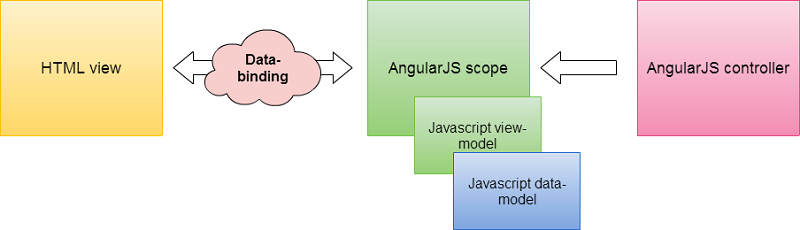
\includegraphics[width=.8\textwidth]{fig/angular-scope}
  \caption{View-controller binding through the scope}
  \captionsetup{font={footnotesize,bf,it}}
  \caption*{source: \url{http://s.codeproject.com/}}
  \label{fig:angularscope}
\end{figure} 

In addition to the mentioned, the framework allows the definition of \textit{Services} and \textit{Directives}. Services are object that can be injected into a controller and have a wide array of uses, from code reusing to data sharing among controllers. Directives on the other side are utilities to manipulate the views and aren  used in the HTML views. One example of such directives is \texttt{ng-click} which is used to specify which operation will be executed when a element on the DOM is clicked.

The MVC in Angular works using a two-way binding. Data is bound to the view through the \texttt{\$scope} object; if a change happens in the view, the data in the models is automatically updated and if a controller modifies the data in the models, the view is automatically updated. An example is shown on listing \ref{lst:angular1}. In this example. when the button is clicked, the function \texttt{change} will be executed, changing the value on the variable \texttt{text} which will automatically update the paragraph on the view.

\begin{listing}\centering
  \begin{minipage}{.6\textwidth}
    \begin{minted}[linenos=true,mathescape,gobble=6]{html}
	     <div ng-controller="ExampleCtrl">
	       <p>{{text}}</p>
	       <button ng-click="change()"> 
	         Change text 
	       </button>
	     </div>
	     <script type="text/javascript>
	       var app = angular.module('exampleApp');
	       app.controller('ExampleCtrl', function($scope){
	         $scope.text = 'No text yet';
	         $scope.change = function(){
	           $scope.text = 'Button has been clicked';
	         };
	       });
	     </script>
    \end{minted}
  \end{minipage}
  \caption{AngularJS example.}\label{lst:angular1}
\end{listing}

\subsection*{Modules}

Similar to NodeJS, Angular provides it's own module system. Modules act as libraries, providing the application with services and directives. The framework does not provide with any tool for installation and management of modules, however, external package manages such as bower\cite{bower} have been built.

There are other tools that offer support for this framework. Yeoman is a widely used tool for scaffolding web applications. It is used to build skeletons for different types of projects such as Angular projects.

For the following modules have been considered:

\begin{description}
\item[\textit{ui-router:}] Since angular is used for developing single page applications, a way to navigate through the views without reloading the full page is needed. Ui-router provides a more complete than the default way of doing this, offering functionality such as nested view and parametrized views.

\item[\textit{ui-bootstrap:}] Twitter Bootstrap is a CSS and JavaScript framework which aims at cutting the web application development time by reducing the amount of time dedicated to creating stylesheets \cite{twbts}. This module provides angular directives and services for manipulating the elements provided by the framework.

\item[\textit{restangular:}] Angular offers a way of querying REST API through the \textit{resources} module, however, it falls short when the functionality offered is more complex than simple CRUD (Create, Read, Update, Delete) operations. Restangular is a library that replaces the default module with a more complete functionality.

\item[\textit{flowjs:}] Uploading images and other kind of files is a harder task in SPAs than in regular web pages. This module helps in the taks of uploading files with a series of angular directives, although it can be used in other applications.

\item[\textit{leaflet-angular:}] Leaflet, detailed in section \ref{sec:leaflet} is a library for creating interactive HTML5 based maps. This module is used to manipulate leaflet maps using a angular directives and services, which is more convenient than the usual way.

\end{description}

\subsection*{Why AngularJS?}

The project involves a good amount of client side JavaScript programming, so it is expected of the application to become quite difficult to manage. Due to this, there is no doubt that some kind of web application development framework is needed.

Some alternatives exist currently, such as Ember or Knockout, however Angular is the most mature of them. The huge community working with this library and the amount of exiting modules are some of the reasons that decline the balance in favor of angular. Other factors include the focus on developing a Single Page Application, which are more mobile friendly than regular web pages; and the amount of learning tools available for the framework. 

\section{Leaflet}\label{sec:leaflet}

Leaflet is a JavaScript library for building mobile friendly interactive maps. It is designed with simplicity, usability and performance in mind and it works efficiently among all major mobile and desktop browsers, taking advantage of HTML5 and CSS3 when it can\cite{leafletjs}.

The library has quickly become one of the most if not the most popular mapping library since it's release in 2011, due to its small size, ease of use and extendability. The example in listing \ref{lst:leaflet1} shows the creation of a map.

\begin{listing}\centering
  \begin{minipage}{.8\textwidth}
    \begin{minted}[linenos=true,mathescape,gobble=6]{javascript}
	     var map = L.map('map');
	     var layer = L.tileLayer('http://{s}.tile.osm.org/{z}/{x}/{y}.png');
	     layer.addTo(map);
    \end{minted}
  \end{minipage}
  \caption{AngularJS example.}\label{lst:leaflet1}
\end{listing}

\subsection*{Layers}

Leaflet works with the concept of Layer. A layer is a visual representation of a geographic feature or set of features. There are three types of layers in the framework: tiles, vectors and layer groups.

\begin{figure}
  \centering
  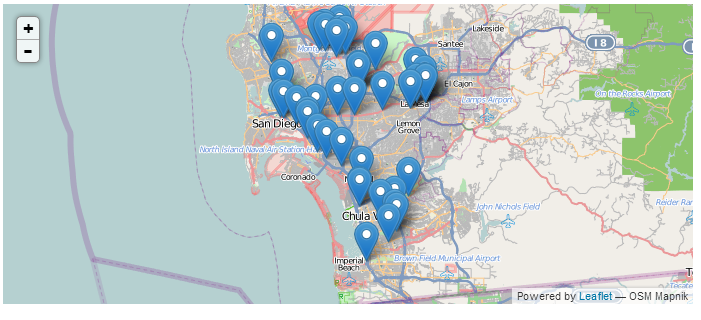
\includegraphics[width=.8\textwidth]{fig/leaflet-osmmapnik}
  \caption{Leaflet with OSM mapnik tile layer}
  \captionsetup{font={footnotesize,bf,it}}
  \caption*{source: \url{http://drupal.org/}}
  \label{fig:leaflet1}
\end{figure} 

\begin{description}
\item[tiles:] Tiles are square bitmap graphics displayed on a grid fashion in order to show a map. Tile layers are defined by a URL from which the images will be obtained and the library will take care of displaying the appropriate grid depending on the zoom level and the view box. The tiles used change drastically the looks of the map, an example of the OSM mapnik tiles can be found in figure \ref{fig:leaflet1}.

\item[vectors:] These layers are used to display information about features on the map in form of geometries. Vector layers can be classified into five categories, three of them corresponding to the typical vector representation on GIS systems: lines, polygons, points, rectangles and circles. Layers can be added and removed from the map easily as shown in example \ref{lst:leaflet2}

\item[layer groups:] The last kind of layers are simply used as a convenience to manipulate more than one feature at the same time. One kind of layer group is the GeoJSON layer which allows the creation of layers from GeoJSON files, detailed in section \ref{sec:geojson}.

\end{description}

\begin{listing}\centering
  \begin{minipage}{.7\textwidth}
    \begin{minted}[linenos=true,mathescape,gobble=6]{javascript}
	     var bounds = [[54.559322, -5.767822], [56.1210604, -3.021240]];
	     L.rectangle(bounds, {color: "#ff7800", weight: 1}).addTo(map);
	     var point = L.marker([50.5, 30.5]);
	     //A popup can be bound to be shown on click
	     point.bindPopup("This is a popup message");
    \end{minted}
  \end{minipage}
  \caption{Leaflet layers.}\label{lst:leaflet2}
\end{listing}

\subsection*{Interaction}

Leaflet is built with the idea of creating interactive maps, thus, it offers methods for manipulating the map and firing and receiving events. It is possible to register listener on map actions, such as when a map is moved or zoomed, or to register listeners on layers, to check when a layer is added, removed, clicked, etc.

This way, it is possible to respond to user actions via callbacks. The framework provides some shortcuts, for example, it is possible to bind the showing of a small popup to the click on a marker without the need to register a callback, as shown in listing \ref{lst:leaflet2}

Another example on the usage of leaflet events can be found in listing \ref{lst:leaflet3}. In the example, a callback is registered for the event of the user moving the map. This is useful for updating the map with information from the layers on the current view.

\begin{listing}\centering
  \begin{minipage}{.5\textwidth}
    \begin{minted}[linenos=true,mathescape,gobble=6]{javascript}
	     // The moveend event is fired every time the
	     // map is moved, dragged or zoomed
	     Map.map.on('moveend', function(){
	       //Obtain the current bounding box of the map
	       var bbox = Map.map.getBounds().toBBoxString();
	       var feature = queryTheServer(bbox);
	       map.addLayer(features);
	     });
    \end{minted}
  \end{minipage}
  \caption{Leaflet layers.}\label{lst:leaflet3}
\end{listing}

\subsection*{Why Leaflet?}

There are not many alternatives when it comes to create JavaScript based maps. Google maps can be used to embed a map on a web page, however, it does not offer much interaction and can hardly be used for other than displaying static data. OpenLayers is another alternative, however, it is known to be hard to learn and the community using it is smaller that Leaflet's one. The amount of developers using leaflet provides the framework with a good deal of extensions and its ease of use make it easy to work with even for novice developers.

\section{Phonegap}\label{sec:phonegap}

Desktop computers are not the only devices that have seen a rise in computational power in the last years, smartphones and other mobile devices have also improved significantly. 

Interaction, screens and even browser support are drastically different in desktop and mobile; and the latter still suffers from a lack of computational power. Due to this web development is not so easily applicable to these devices, building a mobile friendly web application is a difficult task.

However, due to the shift from native to web development happening on desktops, most developers have already learned the tools for developing HTML5 applications. This together with the popularity of mobile apps and difficulty of developing multi-platform applications, has given rise to a number of tools designed to code native mobile applications using HTML5, CSS3 and JavaScript.

The leading among these is Phonegap. Phonegap is a framework that allows to create mobile apps using standardized web APIs for all the major platforms \cite{phonegap}. 

\subsection*{HTML5 development}

The development tools used on a Phonegap application are identical to those used on a regular web page. HTML documents are used to structure the views, CSS stylesheets are used to define the appearance of the application and JavaScript is used to program the behavior.

This is possible because what the library does is opening a enhanced web view (a browser) on the mobile device and loading the files into it. Normally, this would mean that much of the sensors of the device, such as the camera and the gyroscope are not usable, however, the browser created by the framework is extended to allow access to all the hardware on the device.

Phonegap is based on Apache Cordova\cite{apachecordova} which works with a set of plugins. These plugins provide the web view with the functionality it lacks, and expose it as JavaScript APIs. One example of this is the reading of the battery status, as shown on listing \ref{lst:phonegap1}. Aside from the plugins that come shipped with the core libraries, the community has developed a considerable amount of them to provide functionalities that mobile browsers usually lack, such as HTML5 web socket support.

\begin{listing}\centering
  \begin{minipage}{.8\textwidth}
    \begin{minted}[linenos=true,mathescape,gobble=6]{javascript}
	     window.addEventListener("batterystatus", onBatteryStatus, false);
	     
	     function onBatteryStatus(info) {
	         console.log("Level: " + info.level + " isPlugged: " + info.isPlugged);
	     }
    \end{minted}
  \end{minipage}
  \caption{Reading battery status with Phonegap.}\label{lst:phonegap1}
\end{listing}

\subsection*{Phonegap Build}

As convenient using HTML5 for developing cross platform applications is, there is still a need to configure the build for each of the platforms and to install the corresponding Software Development Kits (SDKs) which can be tedious and time consuming.

In the face of this issue, Phonegap offers a platform called Phonegap Build, a cloud based service which helps agile development and allows to compile applications for six of the seven platforms supported by the framework. The Phonegap team illustrated this process in figure \ref{fig:phonegapbuild} on their web page.

\begin{figure}[h]]
  \centering
  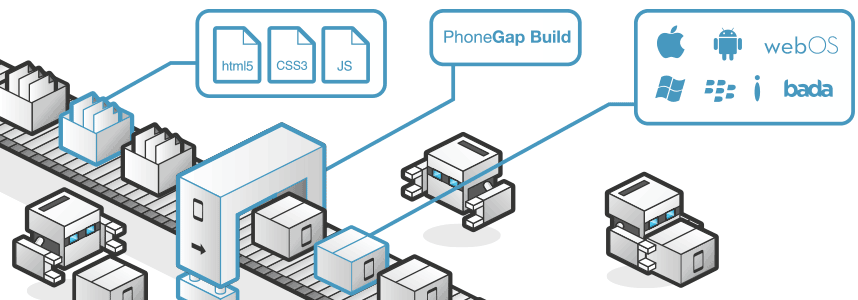
\includegraphics[width=.8\textwidth]{fig/phonegap-build}
  \caption{Phonegap Build process}
  \captionsetup{font={footnotesize,bf,it}}
  \caption*{source: \url{http://phonegap.com/about/}}
  \label{fig:phonegapbuild}
\end{figure} 

\subsection*{Why Phonegap?}

In the world of mobile HTML5 development there are not many competitors. Phonegap is the leading platform, followed by Appcelerator and Ionic. Still, Phonegap is the most mature of them all and has the biggest community, which results in a higher amount of plugins offering more functionality.

On the other side, native development is out of consideration. One of the requirements of the project is for the mobile application to be multi-platform and while developing it natively may increase performance, the payback in development times would be too much. Besides, since the mobile application interfaces and interaction are heavily map based, the code used on other parts of the project can be reused.

Thus, the decision to use Phonegap is made, based on the cut on development times, the re usability of code and the fact that there is no need to learn other development languages.

\section{GPX}\label{gpx}

GPX is a lightweight XML data format for the interchange of GPS data (tracks, routes and way points) between applications and web services on the Internet\cite{gpx}. GPX was released in 2004 and has since then been the de facto standard when it comes to the encoding and interchange of GPS data.

The format represents three types of data, in the following manner:

\begin{description}
\item[Way points:] A way point is a set of coordinates that identifies a point in space. They are represented using the \texttt{<wpt>} tag, as shown in listing \ref{lst:gpx1}

\begin{listing}\centering
  \begin{minipage}{.5\textwidth}
    \begin{minted}[linenos=true,mathescape,gobble=6]{xml}
	     <wpt lat="42.438878" lon="-71.119277">
	       <ele>44.586548</ele>
	       <time>2001-11-28T21:05:28Z</time>
	       <name>Example waypoint</name>
	     </wpt>
    \end{minted}
  \end{minipage}
  \caption{GPX way point representation.}\label{lst:gpx1}
\end{listing}


\item[Tracks:] A track is a segment containing way points, that is, a set of coordinates that describe a path. In GPX tracks are represented by the \texttt{trk} element and point inside one by \texttt{trkpt} elements (see listing \ref{lst:gpx2}).

\begin{listing}\centering
  \begin{minipage}{.5\textwidth}
    \begin{minted}[linenos=true,mathescape,gobble=6]{xml}
	     <trk>
	       <name>Example GPX Document</name>
	       <trkseg>
	         <trkpt lat="47.644548" lon="-122.326897">
	           <ele>4.46</ele>
	           <time>2009-10-17T18:37:26Z</time>
	         </trkpt>
	       </trkseg>
	      </trk>
    \end{minted}
  \end{minipage}
  \caption{GPX track representation.}\label{lst:gpx2}
\end{listing}

\item[Routes:] A route is identical to a track in its encoding, with the difference that the tags \texttt{rte} and \texttt{rtept} are used (see listing \ref{lst:gpx3}). However, there is a difference in the meaning of this concepts; while a track is a record of where a person has been, a route is a suggestion about where someone might go in the future. For this reasons, tracks may have timestamps attached while routes will not.

\begin{listing}\centering
  \begin{minipage}{.5\textwidth}
    \begin{minted}[linenos=true,mathescape,gobble=6]{xml}
	     <rte>
	       <name> Example route </name>
	       <rtept lat="47.644548" lon="-122.326897">
	         <name>Example route point</name>
	       </rtept>
	     </rte>
    \end{minted}
  \end{minipage}
  \caption{GPX route representation.}\label{lst:gpx3}
\end{listing}

\end{description}

\subsection*{Why GPX?}

GPX has been the de facto standard when it comes to representing and interchanging trail and points of interest on the web for ten years. Because of this, it is unreasonable to think in a system which allows interchange of GPS data without using this format. Together with the completeness of the information provided by a GPX file, these are two solid reasons for the usage of GPX on the platform.

\section{GeoJSON}\label{sec:geojson}

GeoJSON is a format for encoding a variety of geographic data structures\cite{geojson}. GeoJSON objects may represent a geometry, a feature or a collection of features (see section \ref{sec:geosparql}, GeoSPARQL). The following geometry types are supported: \texttt{Point}, \texttt{LineString}, \texttt{Polygon}, \texttt{MultiPoint}, \texttt{MultiLineString}, \texttt{MultiPolygon} and \texttt{GeometryCollection}.

More than a file format in itself, it is a specification of how to encode geographical features in JSON format. A complete GeoJSON data structure is always a JSON object, which consists in a collection of key-value pairs, being the key a string and the values any other kind of data.

The specification defines GeoJSON objects in the following way:

\begin{itemize}
\item A GeoJSON object may have any number of members (name/value pairs).
\item The GeoJSON object may have a member with the name \texttt{type}. Its value will be a string that determines the type of the object.
\item The value of the type member must be one of: \texttt{Point}, \texttt{MultiPoint}, \texttt{Polygon}, \texttt{MultiPolygon}, \texttt{LineString}, \texttt{MultiLineString}, \texttt{GeometryCollection}, \texttt{Feature} or \texttt{FeatureCollection}.
\item A GeoJSON object may have an optional member of name \texttt{crs} which specifies the coordinate reference system.
\item A GeoJSON object may have a \texttt{bbox} member, whose value must be a bounding box array.
\end{itemize}

\subsection*{Geometries}

Geometries are GeoJSON objects whose type is different from \texttt{Feature} or \texttt{FeatureCollection}. These elements, unless they are of type \texttt{GeometryCollection}, must have a member of name \texttt{coordinates} which specifies the coordinates of the object in an array of positions.

Positions are represented by an array of numbers, one for the longitude, one for the latitude and an optional one for the elevation, in that order. The coordinates of a object are formed by a array of positions, except for \texttt{Point} element, which have a single position.

A \texttt{GeometryCollection} must have a member named \texttt{geometries}, an array of GeoJSON geometry objects. An example of this can be found on listing \ref{lst:geojson1}.

\begin{listing}\centering
  \begin{minipage}{.6\textwidth}
    \begin{minted}[linenos=true,mathescape,gobble=6]{json}
	      { "type": "GeometryCollection",
	         "geometries": [
	           { "type": "Point",
	             "coordinates": [100.0, 0.0]
	             },
	           { "type": "LineString",
	             "coordinates": [ [101.0, 0.0], [102.0, 1.0] ]
	             }
	         ]
	       }
    \end{minted}
  \end{minipage}
  \caption{A GeoJSON \texttt{GeometryCollection} object.}\label{lst:geojson1}
\end{listing}

\subsection*{Features}

A Feature is a object with some spatial representation. A feature must have two essential members, aside from the type, which are \texttt{geometry} and \texttt{properties}. The first of these members must contain a GeoJSON geometry object, the spatial representation of the object.

The \texttt{properties} member on the other side, is a regular JSON object (a name/value dictionary) and contains all the non-spatial data belonging to the feature. A \texttt{FeatureCollection} does not contain a \texttt{geometry} member, instead it has a \texttt{features} object, an array of feature object in the collection. An example of a feature is shown on listing \ref{lst:geojson2}

\begin{listing}\centering
  \begin{minipage}{.8\textwidth}
    \begin{minted}[linenos=true,mathescape,gobble=6]{json}
	        { "type": "Feature",
	          "bbox": [-180.0, -90.0, 180.0, 90.0],
	          "geometry": {
	            "type": "Polygon",
	            "coordinates": [[
	              [-180.0, 10.0], [20.0, 90.0], [180.0, -5.0], [-30.0, -90.0]
	              ]]
	            },
	            "properties": {
	              "name": "Example feature"
	            }
	          }
    \end{minted}
  \end{minipage}
  \caption{A GeoJSON \texttt{Feature} object.}\label{lst:geojson2}
\end{listing}




